\subsection{Argv Basics}
\begin{itemize}
	\item Arguments are passed to programs as an array too \lstinline[style=C++]{int main(intargc, char *argv[])}
	\item Since each argument is just a sequence of characters, this array is an array of C-strings: \lstinline[style=C++]{char *argv[]}
	\begin{center}
		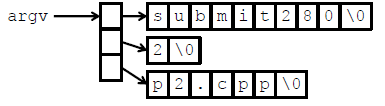
\includegraphics{sections/lec8/argv.png}
	\end{center}
	\item We also need to know how big the array is: \lstinline[style=C++]{int argc}
	\item Suppose we wanted to write a program that is given a list of integers as it’s arguments, and prints out the sum of that list (you'll need to convert the strings to int):
\begin{lstlisting}[style=C++]
intatoi(const char *s);
// EFFECTS: parses s as a number and returns its int value
\end{lstlisting}
\end{itemize}

\subsection{Shell Redirection}
\begin{itemize}
	\item Redirect a file to our program's standard input (cin): \lstinline[style=bash]{./a.out < inputfile>}
	\item Redirect our programs' standard output (cout) to a file: \lstinline[style=bash]{./a.out > outputfile}
	\item This is not File IO, that is done directly instead of the shell.
\end{itemize}

\subsection{File IO}
\begin{lstlisting}[style=C++]
// Open a file using a filestream
string filename = "hello.txt";
ifstreamfilestream;
filestream.open( filename.c_str() );

// CHeck for success opening file
if ( !filestream.is_open() ) {
	cour<< "open failed" << endl;
	exit(1);
}

// Read one word at a time and check that the read was successful
string word;
while ( filestream >> word ) {
	cout<< "word = `" << word << "'\n";
}

// Close file after reading is finished
filestream.close();

/* Alternative: read two words at a time
	string word1, word2;
	while ( filestream>> word1 >> word2 ){
		cout << "word1 = `" << word1 << "'\n"
			 << "word2 = `" << word2 << "'\n";
	}
 */

/* Alternative: read numbers
	int i;
	while (filestream >> i) {
		cout << "i = " << i << endl;
	}
 */
\end{lstlisting}

\subsection{Enums}
\begin{itemize}
	\item Enumeration allows for the categorizing of data
\begin{lstlisting}[style=C++]
enum Month {JAN, FEB, MAR, APR, MAY, JUN,
			JUL, AUG, SEP, OCT, NOV, DEC};
enum Semester {WINTER, SPRING, SUMMER, FALL};

// Define a variable of the new type:
Month this_month;
Semester this_semester;

// Initialize your variables:
this_month = MAY;
this_semester = SPRING;
\end{lstlisting}
	\item Once you have an \lstinline[style=C++]{enum} type defined, you can use it as a function input or output, just like any other type
	\item \lstinline[style=C++]{enum} types are passed by value by default
\end{itemize}

\subsection{Switch statements}
\begin{itemize}
	\item Switch statements work well with enums, and are much faster than long chains of if/else/if/else statements
	\item Two cases with the same result are grouped together since the arms of the case statement ``fall through'' to the next \lstinline[style=C++]{break}
\begin{lstlisting}[style=C++]
Semester s = FALL;
switch(s) {
	case SPRING:
	case SUMMER:
		cout<< "vacation!\n";
		break;
	case FALL:
	case WINTER:
		cout<< "work!\n";
		break;
	default:  // Add a default, just in case
		assert(0); // error!
		exit(1);
}
\end{lstlisting}
\end{itemize}

\subsection{Templates}
\begin{itemize}
	\item The intuition behind templates are that they are code with the ``type name'' left as a (compile-time) constant.
	\item The basic idea of templates is that you declare something to be a template, parameterized across one or more types: \lstinline[style=C++]{template <typename T>}
	\item Then, write the definition of the function you want templated, using the type \lstinline[style=C++]{T} where appropriate:
\begin{lstlisting}[style=C++]
template <typenameT>
	T sum(T a[], intsize) {
	//REQUIRES: T can be initialized to 0 and “+”
	//is defined over T.
	T result = 0;
	for (int i = 0; i<size; ++i)
		result += a[i];
	return result;
}
\end{lstlisting}
	\item Now, we can use this single definition to serve the purposes of both of the ``old'' functions:
\begin{lstlisting}[style=C++]
double a[100] = {... }
intb[200] = {... }
intc[100] = {... }

double aSum= sum(a, 100);
intbSum= sum(b, 200);
intcSum= sum(c, 100);
\end{lstlisting}
	\item How it works:
	\begin{enumerate}
		\item When the compiler sees the first call to \lstinline[style=C++]{sum()}, it inspects the type of the first argument, because that's the ``template type''.
		\item It then generates the code for that version of \lstinline[style=C++]{sum()}, substituting the word \lstinline[style=C++]{double} for the type variable \lstinline[style=C++]{T}. This is called ``instantiation''.
		\item When it sees the second call to \lstinline[style=C++]{sum()}, it does the same thing by generating a second version of \lstinline[style=C++]{sum()} and substituting the word \lstinline[style=C++]{int} for the type variable \lstinline[style=C++]{T}.
		\item When it sees the third call, the compiler knows that that variant of \lstinline[style=C++]{sum()} already exists and simply reuses it.
	\end{enumerate}
\end{itemize}